\section{Data generation}

\subsection{Overview}

This section aims at describing the process that lead to the creation of the dataset, required in order to train the neural network model.

First, an input space is defined, on which will properly select points to form the dataset features. Then, computationally expensive simulation will be run on these points to obtain the desired predicted features for this dataset.

This dataset will afterwards be used to train the surrogate model on \cite{surrogate_model}.

\subsection{Preparatory work}

As stated earlier, this setting only considers the european power system in Dispa-SET, then to create and validate our surrogate model. Each simulation is run over a period of 2019.

\subsubsection{Unit groupings}
In this context, the precise technology and fuel types of each plant is not relevant, as they won't influence the input features of our dataset. Hence, the units are grouped into five categories: flexible units, slow units, storage units, PV units and wind units.

IRENA \cite{irena} describes flexible units as "units that can ramp up and down quickly, have a low minimum operating level and fast start-up and shutdown times", what criterion will be used to separate regular units into the slow and flexible units. This criterion is presented in Table \ref{table:flex-vs-slow-unit}.

\begin{table}[h!]
    \centering
	\begin{tabular}{|l | l | p{8cm}|}
		\hline
		Units & Fuel & Condition \\
		\hline
		$Flex_{units}$ & \multirow{2}{3cm}{GAS, HRD, OIL, BIO, LIG, PEA, NUC, GEO} & $PartLoadMin<0.5$ and $TimeUpMin<5$ and $RampUpRate>0.01$\\ \cline{1-1} \cline{3-3}
		$Slow_{units}$ &  & $PartLoadMin\geq 0.5$ or $TimeUpMin \geq 5$ or $RampUpRate\leq 0.01$\\
		\hline
	\end{tabular}
	\caption{Flexible and slow units classification criterion}
	\label{table:flex-vs-slow-unit}
\end{table}

Refer to Tables \ref{table:technologies-eu} and \ref{table:fuels-eu} for their names.

One also has to consider the limit to the number of hydroelectric units that are possible to build given a geographical area. Given that EU is already almost at saturation, stationary batteries are considered, among other energy storage technology (e.g. compressed air, electric vehicles' battery grid).

As for the other groups, they can be simply described with technology-fuel pairs as follows:
\begin{itemize}
    \item $Storage_{units}$ with (OTH, BATS)
    \item $PV_{units}$ with (SUN, PHOT)
    \item $Wind_{units}$ with either (WIN, WTON) or (WIN, WTOF), the latter not being considered in this work
\end{itemize}

\subsubsection{Parameters estimates}

The availability factors of PHOT and WTON are also required, as well as the peak load. These values are computed from the reference simulation (2019), and are shown in Table \ref{table:param-values}.

\mywarning{needs check}

\begin{table}[h]
    \centering
    \begin{tabular}{|l c c|}
        \hline
        Variable     & Value  & Units \\ \hline
        $AF_{PV}$    & 0.1313 & [$\cdot$]    \\
        $AF_{WTON}$  & 0.2604 & [$\cdot$]   \\
        $PeakLoad$   & 440929 & MW    \\ \hline
    \end{tabular}
    \caption{Values of availability factors and peak load}
    \label{table:param-values}
\end{table}

\subsection{Design space}

\subsubsection{Shape}

The first necessary step in order to select our data points for our dataset, is to define the space in which we will sample them. In our case, this space will be the product of 6 ranges, that is a 6 dimensional hypercube. 

One may argue that some areas of this hypercube, typically around the vertices, will be extremely unlikely to happen in a real setting. More precisely, as this cube will be the input space of the surrogate model that will be connected to another model, it may be suitable to prune the areas of the cube that will never be reached. Indeed, if we know that some areas will never be queried, there is no use covering them.

Furthermore, assuming we would obtain the exact space of possible queries, this space is not likely to be close to some common shape (hypercube, hyperball or combination). Given that most of the design of experiments techniques assume these kinds of space, a mapping would be needed to benefit from the better sampling strategies. Such a mapping would be pretty complex to develop.

More importantly, the cost of being more general than strictly required is small, mainly consisting of a slightly larger surrogate model (in this specific case, a larger neural network), and a larger dataset.

For these reasons, an hypercube will be used.

\subsubsection{Variables}

The six adimensional variables, corresponding to a dimension, are described below, with their given range.

The notation $PowerCap_{x}$ refers to the maximum power output of all the units in $x$. See Table \ref{table:param-values} for the values of the AF and peak load value.

\begin{enumerate}
    \item \textbf{CapacityRatio [$\cdot$]}
    
    Ratio of the maximum production over the maximum demand.
    \begin{equation}
        CapacityRatio  = \frac{PowerCap_{flex units}+Power Cap_{slow units}+PowerCap_{storage units}}{Peak Load}
    \end{equation}

    \item \textbf{ShareFlexibility [$\cdot$]}
    
    Share of the units that are flexible.
    \begin{equation}
        {Share_{flex}}=\frac{PowerCap_{flex units}}{Power Cap_{flex units}+PowerCap_{slow units}}	
    \end{equation}

    \item \textbf{ShareStorage [$\cdot$]}
    
    Ratio of the maximum power output of all storage units over the maximum demand.
    \begin{equation}
        {Share_{storage}}=\frac{PowerCap_{storage units}}{Peak Load}	
    \end{equation}

    \item \textbf{ShareWind [$\cdot$]}
    
    Ratio of the maximum power output of all wind units over the maximum demand.
    \begin{equation}
        Share_{wind}=\frac{PowerCap_{wind units}}{Peak Load}\cdot AF_{WTON}
    \end{equation}

    \item \textbf{SharePV [$\cdot$]}

    Ratio of the maximum power output of all PV units over the maximum demand.
    \begin{equation}
        {Share_{PV}}=\frac{PowerCap_{PV units}}{Peak Load}\cdot AF_{PV}
    \end{equation}

    \item \textbf{rNTC [$\cdot$]}
    
    Net transfer capacity ratio. This variable is a measure of the grid effect on the network, as the zones are able to transmit power between them.

    The data we are provided contains hourly logs of the power transmitted between each pair of zones. The following describes how to compute the rNTC value given these.

    First, we compute the average net transfer capacity (NTC) for each zone $z$ to any other zone $x$ over each of the $N_h$ hours in the input data, via Equation \ref{equation:time-mean-NTC}.

    \begin{equation}
        NTC_{z\rightarrow x} = \frac{1}{N_h} \sum_h NTC_{z\rightarrow x,h}
        \label{equation:time-mean-NTC}
    \end{equation}

    Then Equation \ref{equation:zonal-NTC} is used to compute the zonal NTC, that is the ratio of the sum of all NTCs from this zone to any other zones, over the peak load for that zone.

    \begin{equation}
        NTC_z = \frac{\sum_x NTC_{z\rightarrow x}}{PeakLoad_z}
        \label{equation:zonal-NTC}
    \end{equation}

    A zonal NTC of $1$ for zone $z$ thus means that $z$ would be able, at any time, to fulfill the integrity of its demand by importing electricity from connected zones.

    The final rNTC value is a weighed sum of the zonal NTCs. The weight for a zone $z$ is computed as the ratio of its peak load over the sum of each peak loads. This is expressed by Equation \ref{equation:rNTC}.

    \begin{equation}
        rNTC = \sum_z \frac{PeakLoad_z}{\sum_x PeakLoad_x} NTC_z
        \label{equation:rNTC}
    \end{equation}
\end{enumerate}

\subsubsection{Reference values and ranges}

Given the 2019 input data, a reference simulation is run and one obtains the values presented in table \ref{table:reference-values}.

\begin{table}[h]
    \centering
    \begin{tabular}{|l l l l|}
        \hline
        Variable         & Value  & Lower bound & Upper bound \\ \hline
        CapacityRatio    & 1.658  & 0.5         & 1.8         \\
        ShareFlexibility & 0.418  & 0.01        & 0.99        \\
        ShareStorage     & 0.497  & 0           & 0.5         \\
        ShareWind        & 0.106  & 0           & 0.5         \\
        SharePV          & 0.035  & 0.2         & 0.5         \\
        rNTC             & 0.282  & 0           & 0.7         \\ \hline
    \end{tabular}
    \caption{Values of the different variable for the reference simulation in 2019.}
    \label{table:reference-values}
\end{table}
\mywarning{SharePV c'est un peu optimiste ou il y a un zéro en trop ?}

\subsection{Design of experiments}

A strategy to choose sampling points from some design space is called a design of experiment (DoE). It aims at producing a set of samples that represent as best as possible the entire design space, a property that is required to obtain a well balanced dataset. 

The main methods to acheive such sampling are \cite{doe} illustrated in the following.
\begin{enumerate}
    \item The "naïve" sampling: take samples at regular intervals on the design space. Note that one may not choose the same intervals for different dimensions. It is depicted on Figure \ref{fig:sampling-naive}.
    \item The Monte-Carlo sapling: pick samples at random all over the design space. It is depicted on Figure \ref{fig:sampling-monte-carlo}.
    \item The Latin-hypercube sampling \cite{wiki-lhs}, maximizing a criterion that is either \cite{pydoe-docs}:
    \begin{enumerate}
        \item centering samples in sampling intervals
        \item maximizing the minimum distance between two samples
        \item maximizing the minimum distance between two samples, but place sample in a random location in its interval
        \item minimizing the maximum correlation between two samples
    \end{enumerate}
    These are depicted on Figures \ref{fig:sampling-lhs-center}, \ref{fig:sampling-lhs-maximin}, \ref{fig:sampling-lhs-centermaximin} and \ref{fig:sampling-lhs-corr}.
\end{enumerate}

\begin{figure}[h!]
    \centering
    \begin{subfigure}[b]{0.49\textwidth}
        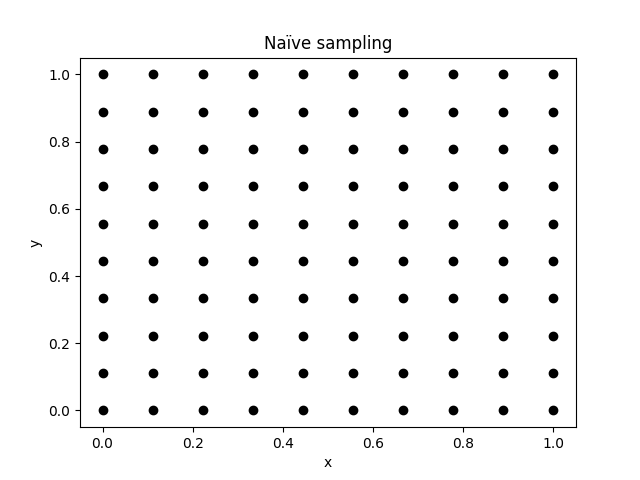
\includegraphics[width=\textwidth]{sampling-naive.png}
        \caption{Naïve strategy}
        \label{fig:sampling-naive}
    \end{subfigure}
    \hfill
    \begin{subfigure}[b]{0.49\textwidth}
        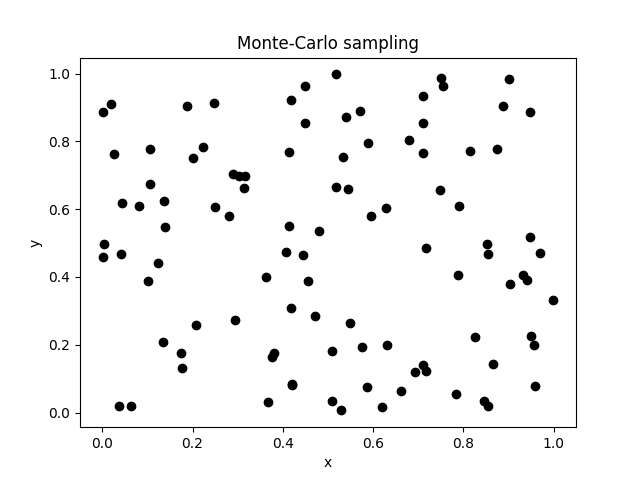
\includegraphics[width=\textwidth]{resources/images/sampling-monte-carlo.png}
        \caption{Monte-Carlo strategy}
        \label{fig:sampling-monte-carlo}
    \end{subfigure}
    \caption{Basic sampling strategies}
\end{figure}

\begin{figure}[h!]
    \centering
    \begin{subfigure}[b]{0.49\textwidth}
        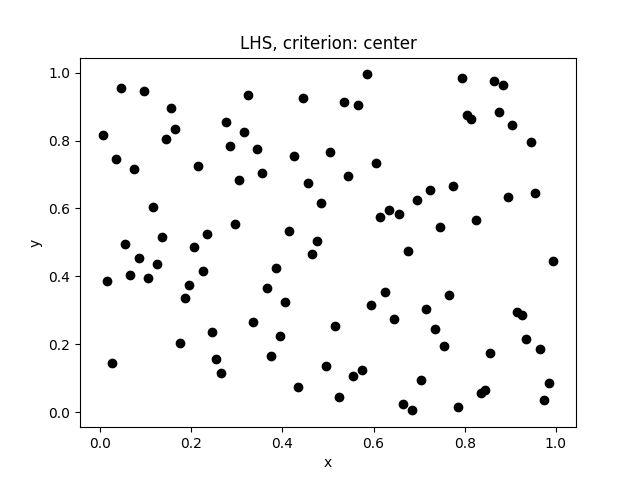
\includegraphics[width=\textwidth]{resources/images/sampling-lhs-center.png}
        \caption{LHS with center criterion}
        \label{fig:sampling-lhs-center}
    \end{subfigure} 
    \hfill
    \begin{subfigure}[b]{0.49\textwidth}
        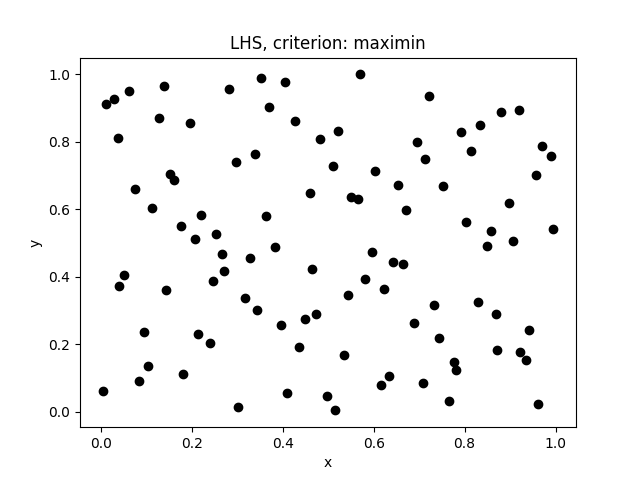
\includegraphics[width=\textwidth]{resources/images/sampling-lhs-maximin.png}
        \caption{LHS with max min distance criterion}
        \label{fig:sampling-lhs-maximin}
    \end{subfigure} 
    \hfill
    \begin{subfigure}[b]{0.49\textwidth}
        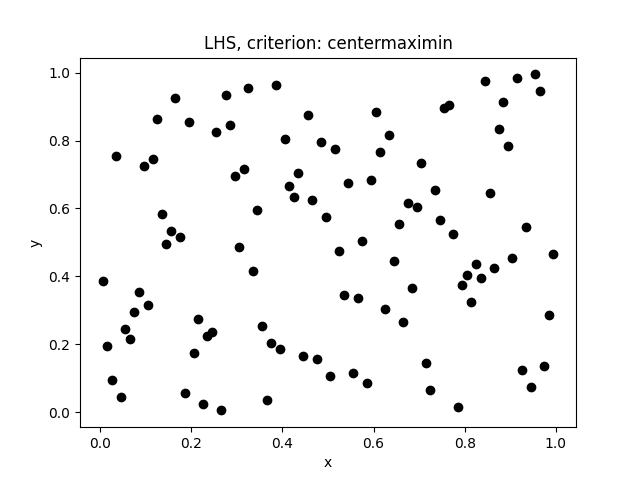
\includegraphics[width=\textwidth]{resources/images/sampling-lhs-centermaximin.png}
        \caption{LHS with max min distance and center criterion}
        \label{fig:sampling-lhs-centermaximin}
    \end{subfigure} 
    \hfill
    \begin{subfigure}[b]{0.49\textwidth}
        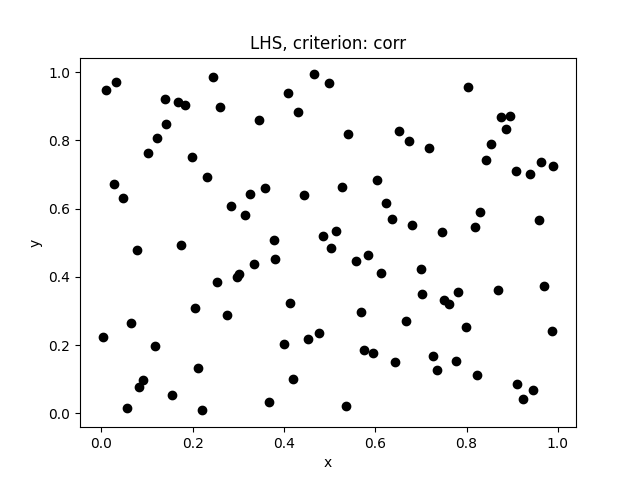
\includegraphics[width=\textwidth]{resources/images/sampling-lhs-corr.png}
        \caption{LHS with correlation criterion}
        \label{fig:sampling-lhs-corr}
    \end{subfigure} 
    \caption{Latin hypercube sampling strategies with every criterion}
\end{figure}

From these 2-dimensional illustration it is clear that the latin hypercube sampling performs best, the naive sampling featuring too much regularities that is not wanted, as they may introduce some bias, and Monte-Carlo sampling tends to make more clusters of samples, that would be inefficient (indeed, making two times the same simulation is useless).

\subsection{Generation of the dataset}

With the input samples now obtained, the next step is now to compute the simulations on each of these points.

But this task is not trivial: we don't have the data that corresponds to these exact configuration. It is thus needed to craft some new simulation settings given a reference, that is the year 2019.

\subsubsection{Adjusting function}
To do so, Dispa-SET disposes of utility functions that do just that, adjusting the capacities, i.e., the power ouputs of the units, in function of some parameters.

These adjusting functions have been specifically developped for this topic by Vidal in her master thesis \cite{carlas-thesis}.

\begin{itemize}
    \item \texttt{adjust\_flexibility} modifies installed capacities to reach the desired $Share_{flex}$.
    
    To do so, it first computes the target capacity, by multiplying the total capacity by the desired $Share_{flex}$. It then add or subtracts the missing or exceeding flexible unit power capacity to each zone, weighting by their total capacity, following Equation \ref{equation:flex-cap-weight}.

    \begin{equation}
        capacity_{z,new} = capacity{z,old} + \frac{capacity_{z,new}}{\sum_x capacity_{x,old}} (target-actual)
        \label{equation:flex-cap-weight}
    \end{equation}

    \item \texttt{adjust\_capacity} applies a linear scaling to the power output of some given set of units, in particular, it will be called multiples times to adjust the storage, PV and wind capacities.
    
    Scaling factors applied are summarized in Table \ref{table:scaling-factors}.

    \begin{table}[h]
        \centering
        \begin{tabular}{|l l|}
            \hline  
            Units              & Scaling factor    \\ \hline
            $Storage_{units}$  & $Share_{storage}$ \\ 
            $Wind_{units}$     & $\frac{CapacityRatio \cdot Share_{wind}}{AF_{wton}}$ \\
            $PV_{units}$       & $\frac{CapacityRatio \cdot Share_{PV}}{AF_{PV}}$ \\ \hline
        \end{tabular}
        \caption{Scaling factors applied to different units}
        \label{table:scaling-factors}
    \end{table}

    \item \texttt{adjust\_rntc} applies a linear scaling to each zonal NTC time series.
\end{itemize}

\subsubsection{Extracted outputs}

As every simulation runs outputs a lot more than only the curtailment and lost load values, some other outputs variables will be extracted from the simulations, while not directly useful for the time being.

Of course, these may reveal themselves useful for future work.

All the outputs extracted from the simulations are displayed in Table \ref{table:values-extracted}.

\begin{table}[h]
    \centering
    \begin{tabular}{|l c|l c|}
		\hline
		Parameter & Unit & Parameter & Unit \\
		\hline
		Cost            & €/MWh & Shedding & TWh \\
		Congestion      & h     & LostLoad & TWh \\
		PeakLoad        & MW    & CF gas  & [$\cdot$] \\
		MaxCurtailment  & MW    & CF nuc  & [$\cdot$] \\
		MaxLoadShedding & MW    & CF wat   & [$\cdot$] \\
		Demand          & TWh   & CF win   & [$\cdot$] \\
		NetImports      & TWh   & CF sun   & [$\cdot$] \\
		Curtailment     & TWh   &  &  \\
		\hline
	\end{tabular}
	\caption{Values extracted from each simulations}
	\label{table:values-extracted}
\end{table}

\subsection{Implementation}

One simple, yet important notice: running all of these simulation is not feasible on a basic hardware. This arises the need for the cluster use, and thus of submitting these as jobs on the cluster.

As the NIC5 cluster provided by CÉCI is obviously shared, one needs to manage the submitted jobs appropriately. In our case, we simply have the same program to be run a bunch of times, that are jobs independent of each other.

\subsubsection{Steps}
For a complete experiment to be completed, these steps have to be followed:
\begin{enumerate}
    \item Generating the reference simulation, to extract the data that will be manipulated by the adjusting function
    \item For each sample, do:
    \begin{enumerate}
        \item Call the adjusting function and create the simulation directory, with all the simulation input data
        \item Call GAMS in this simulation directory
        \item Fetch GAMS outputs in this directory
    \end{enumerate}
\end{enumerate}

\subsubsection{Scripts and code}

The steps presented above almost map to a script or function written. The flow of the dataset generation is as described here.

\begin{enumerate}
    \item The SLURM script \texttt{main.sh} is submitted on the cluster. It fetches relevant data in the \texttt{config.py} script.
    \item It submits the generation of the reference simulation as another job on the cluster and waits for its completion.
    \item It calls \texttt{sampling.py} with argument \texttt{--sample-only}, that will create the \texttt{samples.csv} file containing all the samples.
    \item It prepares the file \texttt{dataset.csv} by writing its header line.
    \item It finally runs the bash script \texttt{launch-job-series.sh}, that will submit some fixed number of sample jobs, as an array, through the SLURM script \texttt{launch-simulation-jobs.sh}.
    \item Each sample job runs:
    \begin{enumerate}
        \item The simulation directory is prepared by calling the \texttt{sampling.py} script with argument \texttt{--prepare-one} and the index of this simulation (it reads the corresponding line in \texttt{samples.csv}).
        \item GAMS is called on the simulation directory.
        \item The simulation results are read with \texttt{read\_results.py --single}, then outputted to \texttt{dataset.csv}.
        \item The simulation directory is cleaned.
    \end{enumerate}
\end{enumerate}

\subsubsection{Technical aspects}

During the creation of this set of scripts, some technical details require specific attention:
\begin{itemize}
    \item The GAMS solver spawns threads for efficiency, the number of threads must not exceed the number of CPUs allocated by SLURM for that job, otherwise it will disturb the whole node on which it is running, including unrelated jobs.
    \item The total amount of each prepared simulation directory is too large to fit on the allocated disk memory on the cluster.
    \item The Dispa-SET ajdusting function do not write adjusted data to a directory if this directory already exists before the function is called
\end{itemize}

\mywarning{Should I write more about the "history" of the scripts ?}

\subsubsection{Dataset fields}

For completeness, all the fields in the created dataset in \texttt{dataset.csv} are shown on Table \ref{table:dataset-fields}.

\begin{table}[h]
    \centering
	\begin{tabular}{|l c|l c|}
		\hline
		Parameter & Unit & Parameter & Unit \\
		\hline
		Cost            & €/MWh & CF nuc        & [$\cdot$] \\
		Congestion      & h    & CF wat         & [$\cdot$] \\
		PeakLoad        & MW   & CF win         & [$\cdot$] \\
		MaxCurtailment  & MW   & CF sun         & [$\cdot$] \\
		MaxLoadShedding & MW   & Capacity ratio & [$\cdot$] \\
		Demand          & TWh  & Share flex     & [$\cdot$] \\
		NetImports      & TWh  & Share sto      & [$\cdot$] \\
		Curtailment     & TWh  & Share Wind     & [$\cdot$] \\
		ENS             & TWh  & Share PV       & [$\cdot$] \\
		CF gas          & [$\cdot$]  & rNTC           & [$\cdot$] \\
		\hline
	\end{tabular}
	\caption{Dataset fields}
	\label{table:dataset-fields} 
\end{table}